\section{Introdução}

Ordenar objetos, de uma maneira geral, é bastante útil pois ajuda a
organizar, buscar de forma rápida, verificar existência, entre outros
aspectos. Em computação isso não é diferente. A ordenação é utilizada em
várias áreas, por exemplo Bancos de Dados. Com isso precisamos sempre de
algoritmos de ordenação que façam o trabalho em menos tempo, consumindo
menos recursos.

\section{Métodos de Ordenação}

Para ordenar dados computacionais precisamos de métodos, que consistem
em procedimentos que dado um conjunto geram uma saída com o próximo
elemento sempre menor ou igual ao anterior, ou vice versa.

Veremos a implementação e estatísticas dos seguintes métodos de
ordenação:

\begin{itemize}
\item
  Bubble Sort
\item
  Selection Sort
\item
  Insertion Sort
\item
  Quick Sort
\item
  Counting Sort
\item
  Bigger Smaller Sort
\end{itemize}
\subsection{Bubble Sort}

Método de ordenação bastante simples de implementar e entender. A ideia
é percorrer um vetor de dados, normalmente números, e verificar de dois
em dois qual o maior. Em caso positivo trocar um com o outro.

\subsubsection{Complexidade}

Para cada elemento é preciso percorrer o vetor, mesmo que o mesmo já
esteja ordenado. Por isso dizemos que o algoritmo é $O(n^2)$.

\subsubsection{Pseudo-código}

Esse método é caracterizado pelo uso de variável auxiliar para fazer o
\emph{swap} ou troca.

\begin{verbatim}
void bubble_sort(V[], n)
begin
    k = n - 1
    for i = 1 to n do
        for j = 0 to k do
            if V[j] > V[j + 1] do
                aux = V[j]
                V[j] = V[j + 1]
                V[j + 1] = aux
            endif
        endfor
    endfor
end
\end{verbatim}
\subsection{Selection Sort}

O algoritmo inicia buscando o valor mínimo e o coloca na primeira
posição. Depois busca o segundo menor valor e o coloca na segunda
posição. Assim por diante.

\subsubsection{Complexidade}

Selecionar o menor elemento requer verificar todos os $n$ elementos
(sendo $n - 1$ comparações) e então colocá-lo na posição correta.
Encontrar o próximo requer uma busca em $n - 1$ elementos. Daí temos:

\begin{equation}
(n - 1) + (n - 2) + \cdots + 2 + 1 = \frac{n (n - 1)}{2} \in \Theta(n^2)
\end{equation}

\subsubsection{Pseudo-código}

Também possui o \emph{swap}, entretanto pode ser que o elemento já
esteja na posição correta, e deverá ser ignorado.

\begin{verbatim}
void selection_sort(V[], n)
begin
    for i = 0 to n - 1 do
        min = i
        for j = i + 1 to n do
            if V[j] < V[min] do
                min = j
            endif
        endfor
        if min != i do
            aux = V[i]
            V[i] = V[min]
            V[min] = aux
        endif
    endfor
end
\end{verbatim}
\subsection{Insertion Sort}

A ideia é, se os primeiros elementos já estão ordenados, um elemento não
ordenado pode ser inserido no conjunto ordenado no lugar adequado.

\subsubsection{Complexidade}

Para inserir o último elemento precisamos de pelo menos $n - 1$
comparações e $n - 1$ movimentos. Para inserir o penúltimo elemento
precisamos de $n - 2$ comparações e $n - 2$ movimentos. E assim por
diante. Daí podemos concluir que teremos:

\begin{equation}
2 \cdot (1 + 2 + 3 + \dots + (n - 1)) = \frac{2 \cdot (n - 1) \cdot n}{2} = (n - 1) \cdot n \in \Theta(n^2)
\end{equation}

\subsubsection{Pseudo-código}

\begin{verbatim}
void insertion_sort(V[], n)
begin
    for i = 1 to n do
        j = i
        while j != 0
                && V[j] < V[j - 1] do
            aux = V[j]
            V[j - 1] = V[j]
            V[j] = aux
            j = j - 1
        endwhile
    endfor
end
\end{verbatim}
\subsection{Quick Sort}

Método caracterizado pelo uso da técnica de divisão e conquista, ou
seja, dividir o problema inicial em subproblemas e resolver um problema
menor utilizando recursividade.

Consiste em dividir o vetor em dois subvetores, dependendo de um
elemento denominado pivô, normalmente o primeiro elemento do vetor. Um
dos subvetores contém os elementos menores que o pivô enquanto o outro
contém os maiores. O pivô é colocado entre ambos, ficando na posição
correta. Os subvetores são ordenados da mesma forma, até que se chegue a
um vetor com um só elemento.

\subsubsection{Complexidade}

Em média o algoritmo é da ordem $O(n \cdot \log n)$, ou seja, há
$\log n$ partições, e para obter cada partição fazemos $n$ comparações
(e não mais que $\dfrac{n}{2}$ trocas).

No pior caso temos $O(n^2)$

\subsubsection{Pseudo-código}

\begin{verbatim}
void quick_sort(V[], initial, final)
begin
    i = initial
    j = final
    pivot = V[(initial + final) / 2]
    while i < j do
        while V[i] < pivot do
            i = i + 1
        endwhile

        while V[j] > pivot do
            j = j + 1
        endwhile

        if i <= j do
            aux = V[i]
            V[i] = V[j]
            V[j] = aux
            i = i + 1
            j = j + 1
        endif
    endwhile

    if j > initial do
        quick_sort(V, initial, j)
    endif

    if i < final do
        quick_sort(V, i, final)
    endif
end
\end{verbatim}
\subsection{Counting Sort}

Diferente de todos os algoritmos vistos até aqui, esse algoritmo não usa
comparações. Para a ordenação é preciso contar quantos elementos existem
e colocá-los num array temporário onde o índice do mesmo é o valor e
cada índice representa o número de vezes que aquele valor aparece.

\subsubsection{Complexidade temporal}

O algoritmo tem tempo de execução de $\Theta(n + k)$, onde $n$ é o
número de elementos a serem ordenados e $k$ é a variação dos tais
números. Se $k = O(n)$, este algoritmo tem performance $\Theta(n)$.

\subsubsection{Complexidade espacial}

A complexidade espacial é $\Theta(n)$, onde $n$ é o tamanho do vetor que
conta os valores. Nenhuma operação de troca é necessária durante o
processo.

\subsubsection{Pseudo-código}

\begin{verbatim}
void counting_sort(V[], n, maxValue)
begin
    count[] = [maxValue + 1]
    for i = 0 to n do
        count[i] = count[i] + 1
    endfor

    z = 0
    for i = 0 to maxValue do
        while count[i] > 0 do
            V[z] = i
            z = z + 1
            count[i] = count[i] - 1
        endwhile
    endfor
end
\end{verbatim}
\subsection{Algoritmo Proposto - Busca do maior e menor}

Inicialmente definimos onde o maior e o menor elementos serão colocados,
usando as variáveis \texttt{ordEsq} e \texttt{ordDir} como visto na
figura \ref{fig:passo1}.

\begin{figure}[h]
   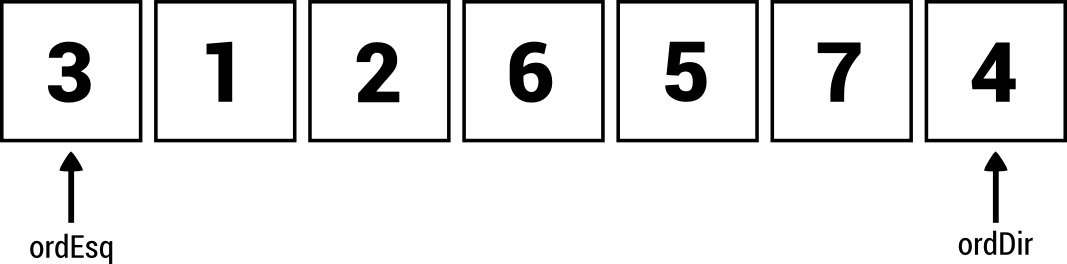
\includegraphics[scale=0.6]{img/maior.menor.algoritmo/passo1.png}
   \caption{definir posicionamento inicial}
   \label{fig:passo1}
\end{figure}

Logo em seguida fazemos uma busca procurando o maior e o menor elementos
(Ver figura \ref{fig:passo2}).

\begin{figure}[h]
   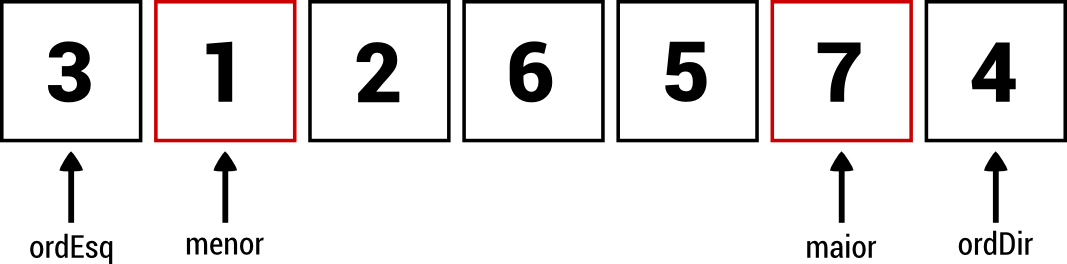
\includegraphics[scale=0.6]{img/maior.menor.algoritmo/passo2.png}
   \caption{busca do maior e menor elementos}
   \label{fig:passo2}
\end{figure}

Ao encontrar devemos trocar o \texttt{menor} com \texttt{ordEsq} e
\texttt{maior} com \texttt{ordDir}. Logo em seguida incrementar o valor
de \texttt{ordEsq} e decrementar o valor de \texttt{ordDir} (Ver figura
\ref{fig:passo3}).

\begin{figure}[h]
   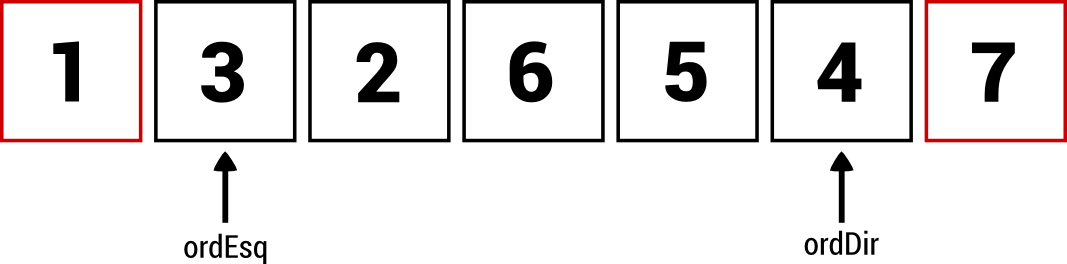
\includegraphics[scale=0.6]{img/maior.menor.algoritmo/passo3.png}
   \caption{tamanho do vetor torna-se $n - 2$}
   \label{fig:passo3}
\end{figure}

\begin{figure}[h]
   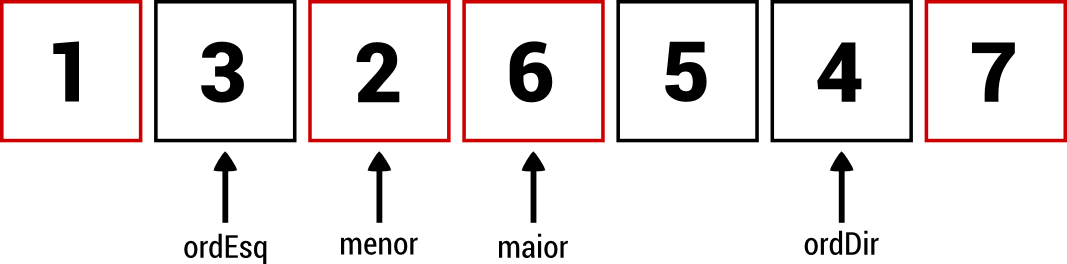
\includegraphics[scale=0.6]{img/maior.menor.algoritmo/passo4.png}
\end{figure}

Notamos que a medida que estamos ordenando, o caminho a percorrer vai
ficando cada vez menor (Ver figura \ref{fig:passo5}).

\begin{figure}[h]
   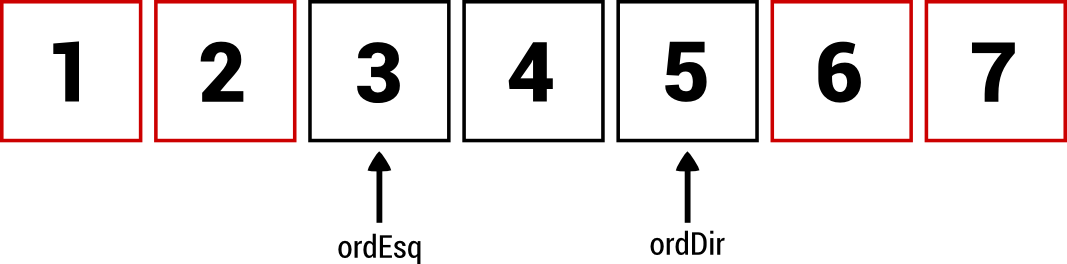
\includegraphics[scale=0.6]{img/maior.menor.algoritmo/passo5.png}
   \caption{tamanho torna-se $n - 4$}
   \label{fig:passo5}
\end{figure}

\begin{figure}[h]
   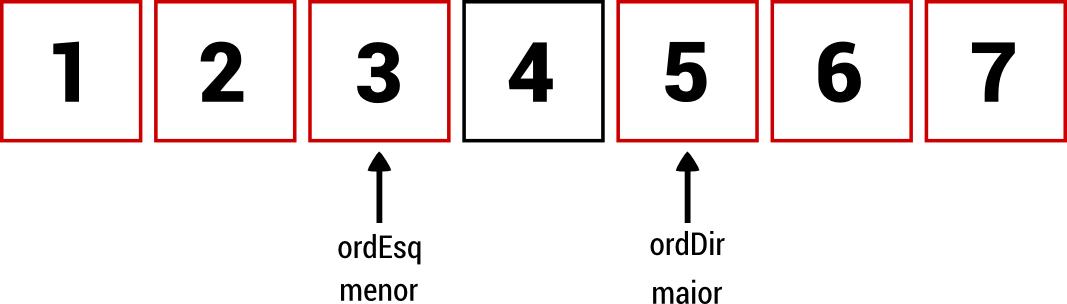
\includegraphics[scale=0.6]{img/maior.menor.algoritmo/passo6.png}
\end{figure}

\begin{figure}[h]
   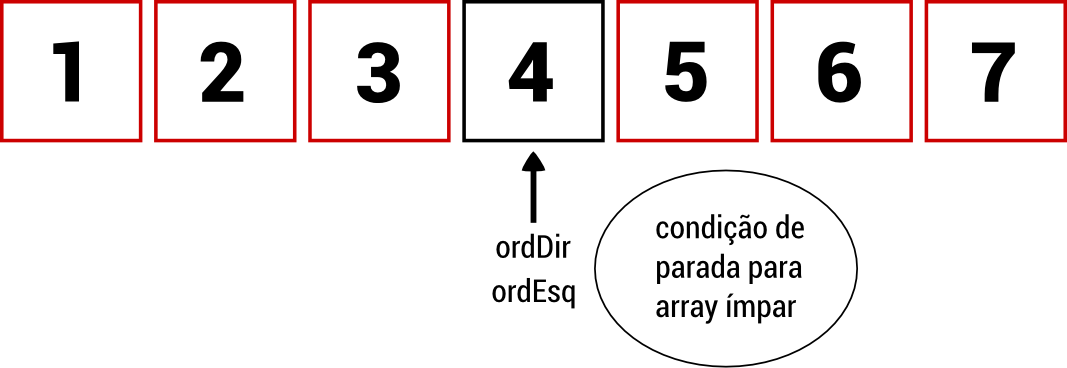
\includegraphics[scale=0.6]{img/maior.menor.algoritmo/passo7.png}
   \caption{vetor ordenado}
   \label{fig:passo7}
\end{figure}

Finalmente, para um \emph{array} ímpar temos que o valor de
\texttt{ordEsq} e \texttt{ordDir} são iguais. Nessa condição não restam
elementos a serem comparados (Ver figura \ref{fig:passo7}).

\subsubsection{Complexidade}

Podemos notar que o algoritmo faz $n$ comparações iniciais. Depois faz
$n - 2$ comparações. Em seguida $n - 4$. E assim por diante.

Podemos criar um conjunto $S = \{2, 4, 6, \dots, n\}$. Dessa forma
podemos dizer que:

\begin{eqnarray*}
T(n) = \sum_{i = 1}^{\frac{n}{2}} S_i
\end{eqnarray*}

\subsubsection{Pseudo-código}

\begin{verbatim}
void maior_menor_sort(V[], n)
begin
    ordEsq = 0, ordDir = n - 1
    for i = ordEsq to (n / 2) do
        maior = i
        menor = i
        for j = i + 1 to ordDir + 1 do
            if V[j] > V[maior] do
                maior = j
            endif

            if V[j] < V[menor]
                menor = j
            endif
        endfor

        if maior != i do
            aux = V[ordDir]
            V[ordDir] = V[maior]
            V[maior] = aux
        endif

        if menor != i do
            aux = V[ordEsq]
            V[ordEsq] = V[menor]
            V[menor] = aux
        endif

        ordEsq = ordEsq + 1
        ordDir = ordDir - 1

        if ordLeft == ordDir do
            break
        endif
    endfor
end
\end{verbatim}
\section{Metodologia}

\subsection{Como os vetores foram gerados}

Os valores do vetor foram gerados usando algoritmo pseudo-randômico em
\emph{python} no seguinte formato:

\begin{itemize}
\item
  \textbf{1° linha}: tamanho do vetor a ser gerado.
\item
  \textbf{restante das linhas}: valores do vetor.
\end{itemize}
O código pode ser encontrado em
\url{https://github.com/atilacamurca/sorty/blob/master/files/gen.py}.

\subsection{Máquina utilizada}

Vejamos a tabela \ref{tab:machine} mostrando detalhes da máquina
utilizada para ordenar os vetores.

\ctable[caption = dados obtidos pelo comando \texttt{lshw} no
Linux.\label{tab:machine}, pos = H, center, botcap]{ll}
{% notes
}
{% rows
\FL
\parbox[b]{0.15\columnwidth}{\raggedright
Classe
} & \parbox[b]{0.67\columnwidth}{\raggedright
Descrição
}
\ML
\parbox[t]{0.15\columnwidth}{\raggedright
system
} & \parbox[t]{0.67\columnwidth}{\raggedright
\texttt{6078AA7}
}
\\\noalign{\medskip}
\parbox[t]{0.15\columnwidth}{\raggedright
bus
} & \parbox[t]{0.67\columnwidth}{\raggedright
\texttt{LENOVO}
}
\\\noalign{\medskip}
\parbox[t]{0.15\columnwidth}{\raggedright
memory
} & \parbox[t]{0.67\columnwidth}{\raggedright
\texttt{2GiB System Memory}
}
\\\noalign{\medskip}
\parbox[t]{0.15\columnwidth}{\raggedright
} & \parbox[t]{0.67\columnwidth}{\raggedright
\texttt{1GiB DIMM DDR2 Synchronous 800 MHz}
}
\\\noalign{\medskip}
\parbox[t]{0.15\columnwidth}{\raggedright
} & \parbox[t]{0.67\columnwidth}{\raggedright
\texttt{DIMM DDR2 Synchronous 800 MHz}
}
\\\noalign{\medskip}
\parbox[t]{0.15\columnwidth}{\raggedright
processor
} & \parbox[t]{0.67\columnwidth}{\raggedright
\texttt{Intel(R) Core(TM)2 Duo CPU E6550 @ 2.33GHz}
}
\\\noalign{\medskip}
\parbox[t]{0.15\columnwidth}{\raggedright
memory
} & \parbox[t]{0.67\columnwidth}{\raggedright
\texttt{16KiB L1 cache}
}
\\\noalign{\medskip}
\parbox[t]{0.15\columnwidth}{\raggedright
} & \parbox[t]{0.67\columnwidth}{\raggedright
\texttt{4MiB L2 cache}
}
\LL
}

\subsection{Estatísticas}

As tabelas abaixo descrevem os algoritmos com seus respectivos tamanhos
dos vetores, médias, valores máximos e mínimos.

\ctable[caption = Vetor de 10 posições., pos = H, center, botcap]{lrrr}
{% notes
}
{% rows
\FL
\parbox[b]{0.25\columnwidth}{\raggedright
Algoritmo
} & \parbox[b]{0.17\columnwidth}{\raggedleft
Média
} & \parbox[b]{0.17\columnwidth}{\raggedleft
Máx.
} & \parbox[b]{0.17\columnwidth}{\raggedleft
Mín.
}
\ML
\parbox[t]{0.25\columnwidth}{\raggedright
Bubble
} & \parbox[t]{0.17\columnwidth}{\raggedleft
0.072
} & \parbox[t]{0.17\columnwidth}{\raggedleft
0.09
} & \parbox[t]{0.17\columnwidth}{\raggedleft
0.09
}
\\\noalign{\medskip}
\parbox[t]{0.25\columnwidth}{\raggedright
Insertion
} & \parbox[t]{0.17\columnwidth}{\raggedleft
0.072
} & \parbox[t]{0.17\columnwidth}{\raggedleft
0.09
} & \parbox[t]{0.17\columnwidth}{\raggedleft
0.09
}
\\\noalign{\medskip}
\parbox[t]{0.25\columnwidth}{\raggedright
Selection
} & \parbox[t]{0.17\columnwidth}{\raggedleft
0.072
} & \parbox[t]{0.17\columnwidth}{\raggedleft
0.09
} & \parbox[t]{0.17\columnwidth}{\raggedleft
0.09
}
\\\noalign{\medskip}
\parbox[t]{0.25\columnwidth}{\raggedright
Quick
} & \parbox[t]{0.17\columnwidth}{\raggedleft
0.072
} & \parbox[t]{0.17\columnwidth}{\raggedleft
0.09
} & \parbox[t]{0.17\columnwidth}{\raggedleft
0.09
}
\\\noalign{\medskip}
\parbox[t]{0.25\columnwidth}{\raggedright
Counting
} & \parbox[t]{0.17\columnwidth}{\raggedleft
0.072
} & \parbox[t]{0.17\columnwidth}{\raggedleft
0.09
} & \parbox[t]{0.17\columnwidth}{\raggedleft
0.09
}
\\\noalign{\medskip}
\parbox[t]{0.25\columnwidth}{\raggedright
Bigger Smaller
} & \parbox[t]{0.17\columnwidth}{\raggedleft
0.072
} & \parbox[t]{0.17\columnwidth}{\raggedleft
0.09
} & \parbox[t]{0.17\columnwidth}{\raggedleft
0.09
}
\LL
}

\ctable[caption = Vetor de 100 posições., pos = H, center, botcap]{lrrr}
{% notes
}
{% rows
\FL
\parbox[b]{0.25\columnwidth}{\raggedright
Algoritmo
} & \parbox[b]{0.17\columnwidth}{\raggedleft
Média
} & \parbox[b]{0.17\columnwidth}{\raggedleft
Máx.
} & \parbox[b]{0.17\columnwidth}{\raggedleft
Mín.
}
\ML
\parbox[t]{0.25\columnwidth}{\raggedright
Bubble
} & \parbox[t]{0.17\columnwidth}{\raggedleft
0.072
} & \parbox[t]{0.17\columnwidth}{\raggedleft
0.09
} & \parbox[t]{0.17\columnwidth}{\raggedleft
0.09
}
\\\noalign{\medskip}
\parbox[t]{0.25\columnwidth}{\raggedright
Insertion
} & \parbox[t]{0.17\columnwidth}{\raggedleft
0.072
} & \parbox[t]{0.17\columnwidth}{\raggedleft
0.09
} & \parbox[t]{0.17\columnwidth}{\raggedleft
0.09
}
\\\noalign{\medskip}
\parbox[t]{0.25\columnwidth}{\raggedright
Selection
} & \parbox[t]{0.17\columnwidth}{\raggedleft
0.072
} & \parbox[t]{0.17\columnwidth}{\raggedleft
0.09
} & \parbox[t]{0.17\columnwidth}{\raggedleft
0.09
}
\\\noalign{\medskip}
\parbox[t]{0.25\columnwidth}{\raggedright
Quick
} & \parbox[t]{0.17\columnwidth}{\raggedleft
0.072
} & \parbox[t]{0.17\columnwidth}{\raggedleft
0.09
} & \parbox[t]{0.17\columnwidth}{\raggedleft
0.09
}
\\\noalign{\medskip}
\parbox[t]{0.25\columnwidth}{\raggedright
Counting
} & \parbox[t]{0.17\columnwidth}{\raggedleft
0.072
} & \parbox[t]{0.17\columnwidth}{\raggedleft
0.09
} & \parbox[t]{0.17\columnwidth}{\raggedleft
0.09
}
\\\noalign{\medskip}
\parbox[t]{0.25\columnwidth}{\raggedright
Bigger Smaller
} & \parbox[t]{0.17\columnwidth}{\raggedleft
0.072
} & \parbox[t]{0.17\columnwidth}{\raggedleft
0.09
} & \parbox[t]{0.17\columnwidth}{\raggedleft
0.09
}
\LL
}

\ctable[caption = Vetor de 1000 posições.,
pos = H, center, botcap]{lrrr}
{% notes
}
{% rows
\FL
\parbox[b]{0.25\columnwidth}{\raggedright
Algoritmo
} & \parbox[b]{0.17\columnwidth}{\raggedleft
Média
} & \parbox[b]{0.17\columnwidth}{\raggedleft
Máx.
} & \parbox[b]{0.17\columnwidth}{\raggedleft
Mín.
}
\ML
\parbox[t]{0.25\columnwidth}{\raggedright
Bubble
} & \parbox[t]{0.17\columnwidth}{\raggedleft
0.08
} & \parbox[t]{0.17\columnwidth}{\raggedleft
0.1
} & \parbox[t]{0.17\columnwidth}{\raggedleft
0.1
}
\\\noalign{\medskip}
\parbox[t]{0.25\columnwidth}{\raggedright
Insertion
} & \parbox[t]{0.17\columnwidth}{\raggedleft
0.086
} & \parbox[t]{0.17\columnwidth}{\raggedleft
0.11
} & \parbox[t]{0.17\columnwidth}{\raggedleft
0.1
}
\\\noalign{\medskip}
\parbox[t]{0.25\columnwidth}{\raggedright
Selection
} & \parbox[t]{0.17\columnwidth}{\raggedleft
0.08
} & \parbox[t]{0.17\columnwidth}{\raggedleft
0.1
} & \parbox[t]{0.17\columnwidth}{\raggedleft
0.1
}
\\\noalign{\medskip}
\parbox[t]{0.25\columnwidth}{\raggedright
Quick
} & \parbox[t]{0.17\columnwidth}{\raggedleft
0.072
} & \parbox[t]{0.17\columnwidth}{\raggedleft
0.09
} & \parbox[t]{0.17\columnwidth}{\raggedleft
0.09
}
\\\noalign{\medskip}
\parbox[t]{0.25\columnwidth}{\raggedright
Counting
} & \parbox[t]{0.17\columnwidth}{\raggedleft
0.072
} & \parbox[t]{0.17\columnwidth}{\raggedleft
0.09
} & \parbox[t]{0.17\columnwidth}{\raggedleft
0.09
}
\\\noalign{\medskip}
\parbox[t]{0.25\columnwidth}{\raggedright
Bigger Smaller
} & \parbox[t]{0.17\columnwidth}{\raggedleft
0.08
} & \parbox[t]{0.17\columnwidth}{\raggedleft
0.1
} & \parbox[t]{0.17\columnwidth}{\raggedleft
0.1
}
\LL
}

\ctable[caption = Vetor de 10000 posições.,
pos = H, center, botcap]{lrrr}
{% notes
}
{% rows
\FL
\parbox[b]{0.25\columnwidth}{\raggedright
Algoritmo
} & \parbox[b]{0.17\columnwidth}{\raggedleft
Média
} & \parbox[b]{0.17\columnwidth}{\raggedleft
Máx.
} & \parbox[b]{0.17\columnwidth}{\raggedleft
Mín.
}
\ML
\parbox[t]{0.25\columnwidth}{\raggedright
Bubble
} & \parbox[t]{0.17\columnwidth}{\raggedleft
0.342
} & \parbox[t]{0.17\columnwidth}{\raggedleft
0.43
} & \parbox[t]{0.17\columnwidth}{\raggedleft
0.42
}
\\\noalign{\medskip}
\parbox[t]{0.25\columnwidth}{\raggedright
Insertion
} & \parbox[t]{0.17\columnwidth}{\raggedleft
0.142
} & \parbox[t]{0.17\columnwidth}{\raggedleft
0.19
} & \parbox[t]{0.17\columnwidth}{\raggedleft
0.16
}
\\\noalign{\medskip}
\parbox[t]{0.25\columnwidth}{\raggedright
Selection
} & \parbox[t]{0.17\columnwidth}{\raggedleft
0.226
} & \parbox[t]{0.17\columnwidth}{\raggedleft
0.29
} & \parbox[t]{0.17\columnwidth}{\raggedleft
0.28
}
\\\noalign{\medskip}
\parbox[t]{0.25\columnwidth}{\raggedright
Quick
} & \parbox[t]{0.17\columnwidth}{\raggedleft
0.128
} & \parbox[t]{0.17\columnwidth}{\raggedleft
0.16
} & \parbox[t]{0.17\columnwidth}{\raggedleft
0.16
}
\\\noalign{\medskip}
\parbox[t]{0.25\columnwidth}{\raggedright
Counting
} & \parbox[t]{0.17\columnwidth}{\raggedleft
0.116
} & \parbox[t]{0.17\columnwidth}{\raggedleft
0.15
} & \parbox[t]{0.17\columnwidth}{\raggedleft
0.14
}
\\\noalign{\medskip}
\parbox[t]{0.25\columnwidth}{\raggedright
Bigger Smaller
} & \parbox[t]{0.17\columnwidth}{\raggedleft
0.244
} & \parbox[t]{0.17\columnwidth}{\raggedleft
0.31
} & \parbox[t]{0.17\columnwidth}{\raggedleft
0.29
}
\LL
}

\ctable[caption = Vetor de 100000 posições.,
pos = H, center, botcap]{lrrr}
{% notes
}
{% rows
\FL
\parbox[b]{0.25\columnwidth}{\raggedright
Algoritmo
} & \parbox[b]{0.17\columnwidth}{\raggedleft
Média
} & \parbox[b]{0.17\columnwidth}{\raggedleft
Máx.
} & \parbox[b]{0.17\columnwidth}{\raggedleft
Mín.
}
\ML
\parbox[t]{0.25\columnwidth}{\raggedright
Bubble
} & \parbox[t]{0.17\columnwidth}{\raggedleft
22.508
} & \parbox[t]{0.17\columnwidth}{\raggedleft
28.14
} & \parbox[t]{0.17\columnwidth}{\raggedleft
28.13
}
\\\noalign{\medskip}
\parbox[t]{0.25\columnwidth}{\raggedright
Insertion
} & \parbox[t]{0.17\columnwidth}{\raggedleft
2.384
} & \parbox[t]{0.17\columnwidth}{\raggedleft
2.98
} & \parbox[t]{0.17\columnwidth}{\raggedleft
2.98
}
\\\noalign{\medskip}
\parbox[t]{0.25\columnwidth}{\raggedright
Selection
} & \parbox[t]{0.17\columnwidth}{\raggedleft
14.128
} & \parbox[t]{0.17\columnwidth}{\raggedleft
17.66
} & \parbox[t]{0.17\columnwidth}{\raggedleft
17.66
}
\\\noalign{\medskip}
\parbox[t]{0.25\columnwidth}{\raggedright
Quick
} & \parbox[t]{0.17\columnwidth}{\raggedleft
0.158
} & \parbox[t]{0.17\columnwidth}{\raggedleft
0.21
} & \parbox[t]{0.17\columnwidth}{\raggedleft
0.19
}
\\\noalign{\medskip}
\parbox[t]{0.25\columnwidth}{\raggedright
Counting
} & \parbox[t]{0.17\columnwidth}{\raggedleft
0.146
} & \parbox[t]{0.17\columnwidth}{\raggedleft
0.19
} & \parbox[t]{0.17\columnwidth}{\raggedleft
0.18
}
\\\noalign{\medskip}
\parbox[t]{0.25\columnwidth}{\raggedright
Bigger Smaller
} & \parbox[t]{0.17\columnwidth}{\raggedleft
10.584
} & \parbox[t]{0.17\columnwidth}{\raggedleft
13.23
} & \parbox[t]{0.17\columnwidth}{\raggedleft
13.22
}
\LL
}

\ctable[caption = Vetor de 1000000 posições.,
pos = H, center, botcap]{lrrr}
{% notes
}
{% rows
\FL
\parbox[b]{0.25\columnwidth}{\raggedright
Algoritmo
} & \parbox[b]{0.17\columnwidth}{\raggedleft
Média
} & \parbox[b]{0.17\columnwidth}{\raggedleft
Máx.
} & \parbox[b]{0.17\columnwidth}{\raggedleft
Mín.
}
\ML
\parbox[t]{0.25\columnwidth}{\raggedright
Quick
} & \parbox[t]{0.17\columnwidth}{\raggedleft
0.318
} & \parbox[t]{0.17\columnwidth}{\raggedleft
0.4
} & \parbox[t]{0.17\columnwidth}{\raggedleft
0.39
}
\\\noalign{\medskip}
\parbox[t]{0.25\columnwidth}{\raggedright
Counting
} & \parbox[t]{0.17\columnwidth}{\raggedleft
0.242
} & \parbox[t]{0.17\columnwidth}{\raggedleft
0.31
} & \parbox[t]{0.17\columnwidth}{\raggedleft
0.3
}
\LL
}

\subsection{Gráficos}

Vamos ver uma comparação com vetores de tamanho variando de 10 a 1000.
Podemos notar que inicialmente todos tendem a levar o mesmo tempo na
média como visto na figura \ref{fig:chart1}. Entretanto a partir do 1000
eles começam a modificar significamente o tempo de execução médio.

\begin{figure}[b]
   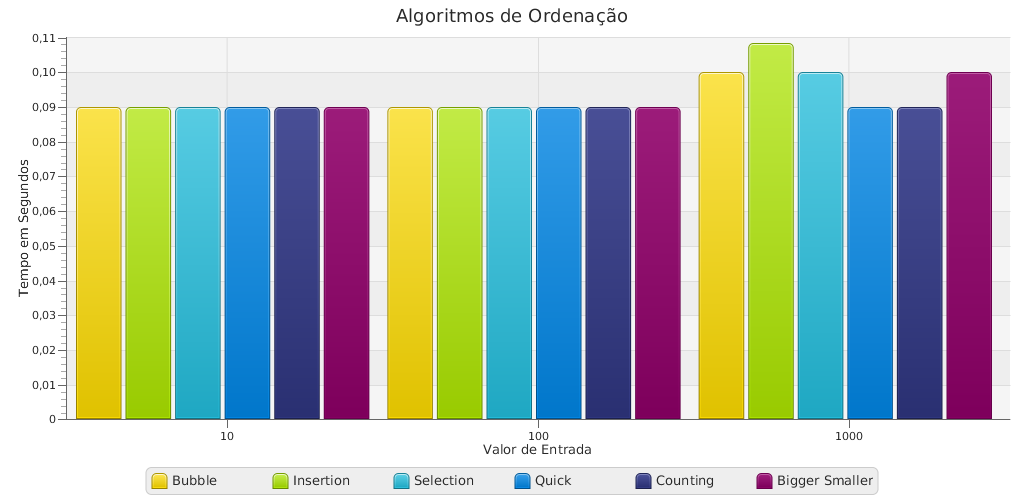
\includegraphics[scale=0.47]{img/charts/chart-1.png}
   \caption{Comparação 10 a 1000}
   \label{fig:chart1}
\end{figure}

Analisando agora vetores de tamanho variando de 1000 a 10000 veremos uma
mudança mais brusca no tempo de execução dos algoritmos, exceto os
algoritmos Quick Sort e counting Sort que são logarítmicos e tendem a
manter seu tempo de execução baixo (figura \ref{fig:chart2}).

\begin{figure}[h]
   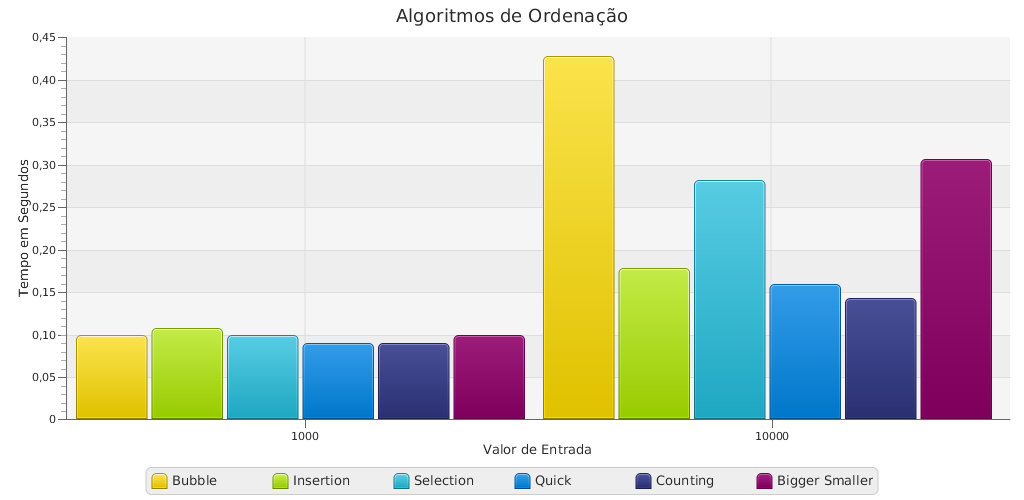
\includegraphics[scale=0.47]{img/charts/chart-2.png}
   \caption{Comparação 1000 a 10000}
   \label{fig:chart2}
\end{figure}

Chegamos a comparação de tamanhos grandes e podemos notar que a
diferença de tempo dá um salto bastante significativo para algoritmos
quadráticos, mas ainda assim Quick Sort e Counting Sort se mantém
(figura \ref{fig:chart3}).

\begin{figure}[h]
   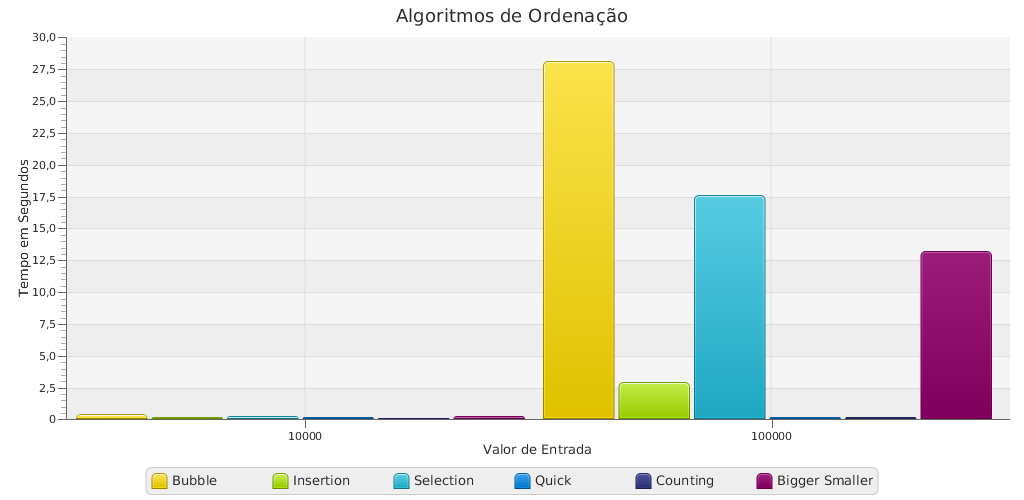
\includegraphics[scale=0.47]{img/charts/chart-3.png}
   \caption{Comparação 10000 a 100000}
   \label{fig:chart3}
\end{figure}

Vamos olhar de perto o Quick e Counting Sort mostrados na figura
\ref{fig:chart4}. Podemos notar que o Counting Sort cresce mais lento
que o Quick Sort. Com isso chegamos a conclusão que comparação de
valores leva um pouco mais de tempo que outras operações, entretanto o
algoritmo Counting Sort usa um vetor adicional, que neste caso tinha
tamanho 100 (todos os vetores possuem valores variando de 0 a 99).

\begin{figure}[h]
   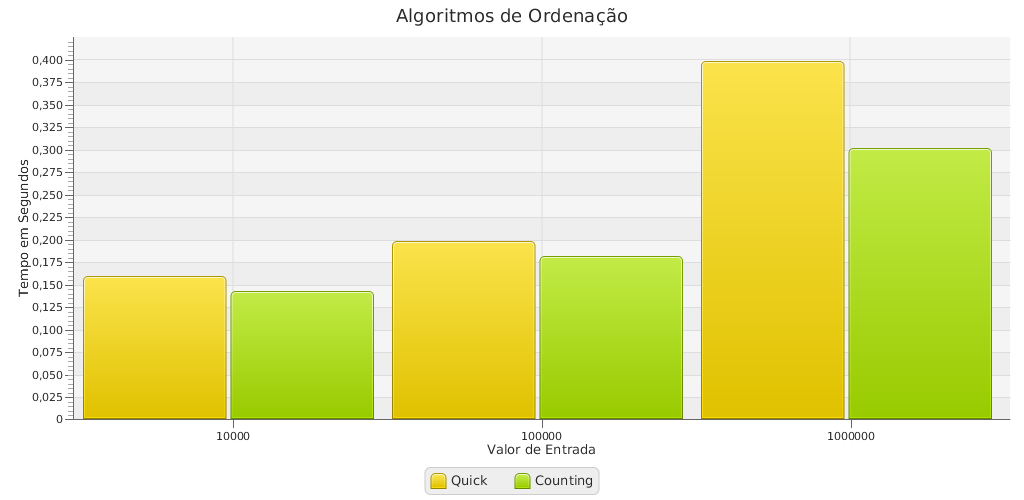
\includegraphics[scale=0.47]{img/charts/chart-4.png}
   \caption{Comparação 10000 a 1000000}
   \label{fig:chart4}
\end{figure}
